%\documentclass[english, a4paper]{article}
\documentclass{llncs}
\usepackage{llncsdoc}

\usepackage{float}
\usepackage[pdftex]{graphicx}
\usepackage[font={small,it}]{caption}
\usepackage[caption=false]{subfig}
\usepackage{url}
\usepackage{siunitx}
\usepackage{graphicx}
\usepackage{pbox}
\usepackage{placeins}

\newcommand{\squeezeup}{\vspace{-8.9mm}}
\setcounter{secnumdepth}{3}
\addtolength{\textfloatsep}{-3mm}
\addtolength{\belowcaptionskip}{-15pt}



\title{Data Mining -- Assignment 2}

\author{Andrew Bedard (2566978) -- Artagan Malsagov (2562231)  -- Shabaz Sultan(2566703)}

\institute{}
\begin{document}
\maketitle
\section{Introduction}
The online travel agency (OTA) Expedia posed the challenge to rank hotels by their likelihood of being booked. In such a competitive market as the one of click-through purchases, properly ranking offered hotels according to user's preferences becomes indispensable for the OTA to win the sale. This requires an algorithm that can rank the hotels associated with a user search query. The use of ranking algorithms in the industry of online travel booking is uncharted territory and the challenge provided opportunities to explore. For further information on the competition see the Kaggle platform \cite{WinNT}.

This report details our approach to tackling this problem based on the search and click-through data provided by Expedia. First, a short review of the available literature on the topic is given. Then a description of the data is provided and the problem is defined in more rigorous terms. This is followed up by a review of the methods and models used by us and how they held up to the challenge. Finally, we finish off with a summary and some concluding remarks.  

\section{Related work}
Here is a sample of the approaches of some of the groups that participated in the Expedia challenge.

Let's start with the official winner of the competition, whose approach can be found in \cite{WinNT2}. For the feature engineering missing values were said to be imputed by negative values, which we believe to mean the worst case is assumed. The rationale being customers don't like to book hotels with missing values. Numerical variables were bounded to remove outliers. Negative instances of booking and clicking were down-sampled. All original features were used, plus engineered features such as averages of numerical variables, price difference and categorical features converted to numerical ones. As a model an ensemble of Gradient Boosting Machines was used. 

The official runner-up also did a lot of feature engineering. Missing values were replaced by worst-case scenarios by the same reasoning as above. For instance the missing values of competitor descriptions where replaced by zero, which means data is not available. Furthermore, certain numerical features were normalized with respect to different indicators such as the prop\_id, srch\_id and month. New features were constructed such as the difference between the visitor's starrating and the starrating given to a certain property. This gave a total of 300 features on which the models LambdaMART, SVM Rank and linear regression were used. The final model used was LambdaMART.

The paper \cite{DBLP:journals/corr/LiuXZYPLSW13} details an approach which meshes together several different ranking models: logistic regression, support vector machines, random forest, gradient boosting machine, factorization machine and LambdaMART, among others. The team identified the most import features as price\_usd, prop\_starrating and prop\_location\_score2. Data was balanced for training random forest, making it feasible to train with a large number of trees.  For missing values the first quartile calculated for the prop\_id of the missing data point was used. As their ensemble the team tried different linear combinations and sought the combination that would give a better result than a single model could.  

 
\section{Problem formulation and data description}
Given a search query $x_{i}$ and the hotels $\{h_{1}^{i},\dots,h_{m_{i}}^{i}\}$ associated with it, where $\leq m_{i} \leq 38$(the maximum number of hotels associated with any search query is not more than $38$ and not less than $4$), a ranking algorithm has to estimate the scores  $\{s_{1}^{i},\dots,s_{m_{i}}^{i}\}$ corresponding to these hotel. The scores are assigned as:
$$
s_{j}^{i}=
\left\{
	\begin{array}{ll}
		5  & \mbox{if hotel $j$ was booked }   \\
		1 & \mbox{if hotel $j$ was clicked }  \\
		0 & \mbox{if hotel $j$ was neither clicked nor booked}
	\end{array}
\right.
$$
  
The data taken from Kaggle totals about $10$ million records spanned by $336,334$ search queries, meaning at least $4$ records correspond to one search query and at most $38$. The data is divided in half into a training and test set. Each record in the training data is represented by $54$-dimensional vector, where the two class variables booking and clicking and the variables for purchase amount and position in Expedia's ranked list are not included in the test set. Indeed, in our problem the target variables to be estimated are click\_bool and book\_boolean, based on which the scores for the ranking can be assigned. The remaining $50$ variables are roughly divided into search criteria, hotel characteristics (dynamic/static), history of the user and competitive OTA information. A variable not covered by these categories is whether the search result were presented in random order or based on the ranking algorithm employed by Expedia (in some cases hotels were presented in random order to learn about user preferences).

As an evaluation metric the average NDCG over all queries is used, with $k=38$ as the truncation level. Formally, $\displaystyle DCG_{k}=\sum_{i=1}^{k}\frac{2^{rel_i}-1}{\log_{2}(i+1)}$. Here $rel_{i}$ represent the true score of the hotel ranked in position $i$. Observe that only one score can be $5$: the hotel booked. The further down the summation it is placed the more it is discounted, decreasing the score. Likewise for the hotels that were clicked and it doesn't matter in which order the clicks are placed, as long as they are ranked below the booked hotel and above the hotels booked nor clicked. The ideal ranking then gives the maximal discounted gain, $IDCG_{k}$. Consequently, $NDCG_{k}=\frac{DCG_{k}}{IDCG_{k}}$         

\section{Working on the data}

	There were a few challenges with working on the data. First was the sheer number of records, thus from the data set approximately 10\% was selected for analysis and training. This was done by first selecting 10\% of the records, then adding further records to ensure we had complete data for each search id, that is, if we selected a record from search id \textit{x}, then all records from search id \textit{x} were added to our data.

	The second large challenge was that many of the records were incomplete. Certainly we can see in figure \ref{fig:pctM}, many of the features were missing over 80\% of their values.
	\begin{figure}[H]
	\centering
	\textbf{Percentage of missing data}\par\medskip
		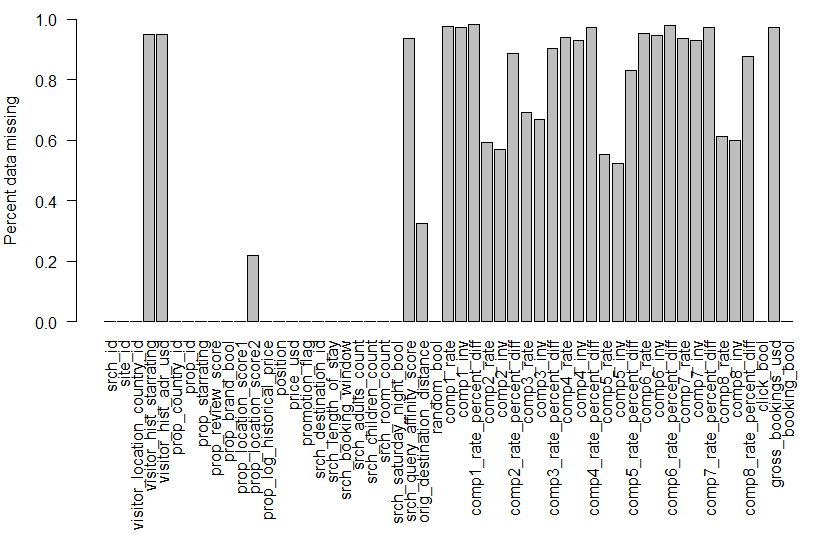
\includegraphics[scale=0.4]{figures/pct_missing.png}
	\caption{Percentage of missing data}
	\label{fig:pctM}
	\end{figure}
	
	Further, there were outliers in some factors, \textit{price\_ usd} for example in our training set had a minimum of 0 and a maximum of 371493.6, it is impossible to tell exactly how this happened or what these represent, however the points were treated as outliers and replaced. Simply applying experimentation we were able to arrive at a formulation for filling in missing or zero values to maximize the NDGC for our final model, they are as follow:
	\begin{itemize}
	\item \textit{price\_ usd} outliers, these were replaced with the first quantile value
	\item missing values in \textit{prop\_ location\_ score2, visitor\_ hist\_ adr\_ usd, visitor\_ hist\_ starrating, prop\_ review\_ score} were replaced with the mean values of each property within their country id. 
	\item Zero values in \textit{prop\_ starrating, prop\_ review\_ score, prop\_ starrating} were replaced with the third quantile values within their country id.
	\item Zero values in \textit{prop\_ log\_ historical\_ price} were replaced by first quantile values. Zero values of \textit{srch\_ length\_ of\_ stay} were replaced with mean within country id.
	\end{itemize}

\[\textit{ump = exp(prop\_ log\_ historical\_ price) - price\_ usd}\]
\[\textit{price\_ diff = visitor\_ hist\_ adr\_ usd - price\_ usd}\]
\[\textit{starrating\_ diff = visitor\_ hist\_ starrating - prop\_ starrating}\]
\[\textit{per\_ fee} = \frac{\textit{price\_ usd*srch\_ room\_ count}}{\textit{srch\_ adults\_ count+srch\_ children\_ count}}\]
\[\textit{score2ma = prop\_ location\_ score2*srch\_ query\_ affinity\_ score}\]
\[\textit{total\_ fee = price\_ usd*srch\_ room\_ count}\]
\[ \textit{score1d2} = \frac{\textit{prop\_ location\_ score2} + 0.0001}{\textit{prop\_ location\_ score1} + 0.0001}\]

	\begin{figure}[H]
	\centering
	\textbf{Correlations}\par\medskip
		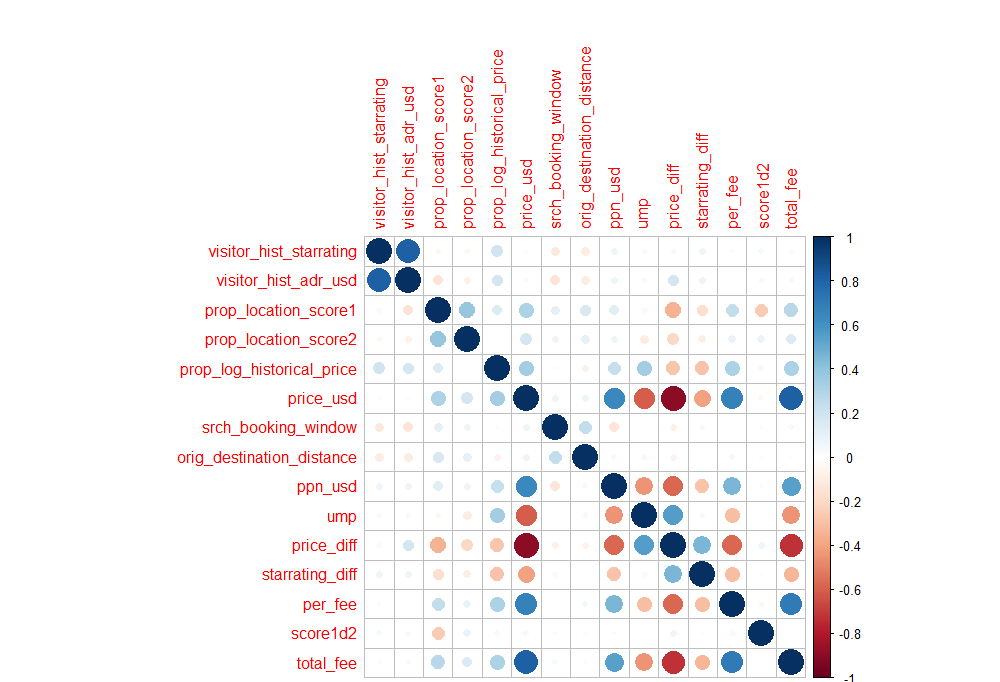
\includegraphics[scale=0.3]{figures/corr_plot.png}
	\caption{Correlations}
	\end{figure}


\section{Models and evaluation}

\subsection*{Artagan}

\subsection*{Andy}

Approach was to follow Liu paper for data pre-processing and logistic regression model.

Most data included large percentage of noise and missing data, use data as outlined in paper, so \textit{prop\_ location\_ score2, ump, price\_ diff, starrating\_ diff, score1d2, random\_ bool, per\_ fee, price\_ usd, prop\_ review\_ score, total\_ fee, prop\_ starrating}

After pre-processing, a clicking classifier was created using Logistic Regression in sklearn with class\_ weight being set to auto to ensure that negative instances were weighted down, this classifier was then fit to our model using the training data 10\_ pct.

This process was repeated creating a booking classifier.

Calculated NDGC for all features give: 0.353067825035
Calculated NDGC for using features in the end: 0.380235534251



\subsubsection*{Mr. Get'er done}


          
\bibliographystyle{plain}
\bibliography{report}
\end{document}
